\documentclass{report}
\pagenumbering{arabic}
\setcounter{chapter}{1}
\usepackage{titlesec}           % ← For custom section numbering
\usepackage[margin=3cm]{geometry}
\usepackage{tocbibind}
\usepackage{array}

\usepackage{tikz}
\usepackage{float}
\usepackage{subcaption}
\usetikzlibrary{arrows.meta,positioning,calc,shapes.geometric}
% Format: "1. Heading" style
\titleformat{\section}
  {\normalfont\Large\bfseries}  % Font
  {\thesection}                % "1." format  
  {1em}                         % Space after number
  {}                            % Title


\title{\textbf{Fire Alarm using Flame Sensor and BC557 Transistor}}
\author{Sounak Mal (12200323050) \\ Jagannath Maji (12200323024) \\ Pradip Mandal (12200323031) \\ Ritankar Mandal (12200323037)}
\date{}

%!TEX root = main.tex

\begin{document}

\maketitle

\section{Abstract}
The advancement of technology has led us to both new opportunities and challenges. One of the major challenges is ensuring safety in our homes and workplaces. Fire alarms play a crucial role in alerting us to potential fire hazards, allowing us to take necessary precautions. In this project, we have designed a fire alarm system using a flame sensor, a BC557 transistor, and a buzzer. The flame sensor detects the presence of fire by sensing the infrared light emitted by flames, while the BC557 transistor amplifies the signal from the flame sensor to trigger an alarm and activate a buzzer when a fire is detected. The buzzer provides an audible alert, ensuring immediate attention. The system is designed to be cost-effective and easy to maintain, making it accessible to a wide range of users. The results obtained from both simulation and practical implementation show that the fire alarm system is reliable and efficient in detecting fire hazards, providing an effective solution for enhancing safety in various settings.

\section{Introduction}

In the age of technology, safety is of utmost importance. Fire alarms play a crucial role in ensuring the safety of individuals and property. In this project, we have designed a fire alarm system using a flame sensor, a BC557 transistor, and a buzzer. The flame sensor detects the presence of fire by sensing the infrared light emitted by flames. The BC557 transistor is used to amplify the signal from the flame sensor and trigger an alarm and activate a buzzer when a fire is detected. The buzzer provides an audible warning, making the system more effective in alerting people to fire hazards.

The main objective of this project is to create a reliable and efficient fire alarm system that can be easily implemented in homes, offices, and other buildings. The system is designed to be cost-effective and easy to maintain, making it accessible to a wide range of users.

Several projects have been developed under this topic for constructing a fire alarm system using different components. A fire alarm circuit has been done on detecting forest fires by optimally placing the fire sensors, which reduces interference. The report proposes optimal placement of the fire detection sensors based on the signal-to-interference-plus-noise ratio criterion. The proposed approach is analytically evaluated, and the results show that the throughput is 53.28\% compared to the random deployment of sensors, where the throughput is 45.21\% [1]. Another work has been proposed on designing of a voltage tunable dual band Ge-on-Si photodector combining wavelength sensitive detection with classification algorithms.The  evaluation and its performance against various interference sources, by exploiting machine learning models such as Support Vector Machines (SVM) and Quadratic SVM, has achieved up to 99.8\% classification accuracy [2]. There is a report on proposal of how to reduce false alarms on benign flames using 3D CNNs. The study primarily relies on how bright illumination or presence red colored objects can cause false alarms. By the application FalseNet, a new video dataset, consisting of both real and fires and common false-positive sources.Paired with a 3D ResNet+(2+1)D CNN using CBAM attention, it achieves 90.44\% accuracy by better distinguishing benign flames from actual fire hazards in CCTV footage. Grad-CAM confirms the model focuses on correct spatial features [3]. Another project focuses on a rTPNN (Recurrent Trend Predictive Neural Network) which is a novel multi-sensor fire detection model that predicts both sensor level and trend patterns using recurrent processing, which achieves 96\% accuracy, outperforms LSTM/SVM/MLP (both TP/TN $>92\%$), and triggers alarms in 11s (vs 22s for others). Ideal for real-time fire detection [4].
A Privacy-Preserving Iot-Based Fire Detector proposes on a privacy preserving IoT fire detection system which extracts video data from raw footage and sends to the cloud for analysis,achieving 97.5\% accuracy using binary video descriptors + CNN. Outperforms raw video methods while protecting privacy. Runs real-time on Raspberry Pi 4 (100\,ms/frame) [5].

In this paper, we will discuss about the design of the fire alarm system, by the use of a flame sensor and a BC557 transistor. The discussion will include the working principle of the components used, the results obtained and future scope of this project. The results are both simulated in TinkerCAD, (a simulation program by Anydesk) and practically implemented in the Laboratory.

\section{Literature Overview}

\begin{itemize}
	\item[{\bf [1]}] Z. Shafiq \textit{et al.}, ``Optimal Placement of Fire Detection Sensors for Reduced Interference in Wireless Sensor Networks,'' \textit{IEEE Open Journal of the Communications Society}, vol. 6, pp. 9304--9321, 2025, doi: 10.1109/OJCOMS.2025.3626689. \\
	      \textit{keywords:} Sensors; Forestry; Wireless sensor networks; Interference; Wildfires

	\item[{\bf [2]}] R. Elagib \textit{et al.}, ``Flame Detector Based on a Ge-on-Si Photodetector With a Voltage Tunable Spectral Response,'' \textit{IEEE Access}, vol. 13, pp. 174071--174077, 2025, doi: 10.1109/ACCESS.2025.3618306. \\
	      \textit{keywords:} Fires; Photodetectors; Detectors; Machine learning; Flame detection

	\item[{\bf [3]}] M. M. E. H. Ali and M. Ghodrat, ``Toward Reliable Fire Detection in Indoor CCTV Footage: Reducing False Alarms From Benign Flames Using 3D Attention CNNs,'' \textit{IEEE Access}, vol. 13, pp. 144092--144103, 2025, doi: 10.1109/ACCESS.2025.3598919. \\
	      \textit{keywords:} Fires; Videos; Object detection; False alarms; Smart buildings

	\item[{\bf [4]}] M. Nakip \textit{et al.}, ``Recurrent Trend Predictive Neural Network for Multi-Sensor Fire Detection,'' \textit{IEEE Access}, vol. 9, pp. 84204--84216, 2021, doi: 10.1109/ACCESS.2021.3087736. \\
	      \textit{keywords:} Detectors; Neural networks; Multi-sensor; Sensor fusion; Fire detection

	\item[{\bf [5]}] A. H. Altowaijri \textit{et al.}, ``A Privacy-Preserving IoT-Based Fire Detector,'' \textit{IEEE Access}, vol. 9, pp. 51393--51402, 2021, doi: 10.1109/ACCESS.2021.3069588. \\
	      \textit{keywords:} Videos; Feature extraction; IoT devices; Temperature sensors; Privacy
\end{itemize}

\section{Project Workflow}

\subsection{Researching and Conceptualization}
In this phase, we conducted extensive research on fire alarm systems, focusing on the components and technologies that could be used to create an effective and reliable system. We explored various types of journals and articles related to fire detection, sensor technologies, and circuit design. This research helped us to conceptualize the design of our fire alarm system using a flame sensor and a BC557 transistor.

\subsection{Components Selection}
In this phase, after doing extensive research on the topic, the components are selected based on their functionality and availability. The components include a flame sensor for detecting flames, a BC557 transistor, a resistor to limit the current, a blue LED to indicate the presence of fire, a buzzer for audible alert, and a battery to power the circuit.

\subsection{Software Simulation Approach}
In this phase, we used TinkerCAD, a simulation software, to design and test our fire alarm circuit. We created a virtual circuit using the selected components and simulated the operation of the fire alarm system. This allowed us to verify the functionality of our design and make any necessary adjustments before moving on to practical implementation.

\subsection{Practical Implementation}
The fire alarm circuit was the implemented in this phase. The components are all assembled on a breadboard, and the circuit is tested to ensure that it works as intended. We observed the behavior of the circuit when exposed to a flame and verified that the LED indicator turns on, signaling the detection of fire.

\subsection{Calibration \& Adjustment}
After the initial implementation, the calibration of the flame sensor was done to ensure that it accurately detect flames. The adjustment of sensitivity of the sensor is done and then tested the circuit under different conditions to ensure that it responds correctly to the presence of fire.

\subsection{Testing and Results}
Then, the testing of the fire alarm system is conducted thoroughly to evaluate its performance. Different flame sources were exposed to the circuit and the response of the LED indicator is observed. The results showed that the fire alarm system successfully detected flames and provided a reliable alert mechanism.

\subsection{Data Collection}
During the testing phase, data was collected on the response time of the fire alarm system, the sensitivity of the flame sensor, and the overall reliability of the circuit. This data was analyzed to assess the performance of the fire alarm system and identify any areas for improvement.

\subsection{Documentation \& Reporting}
Finally, the entire project process, including the design, implementation, testing, and results, is documented in a comprehensive report. This report includes detailed explanations of the components used, the circuit design, the testing procedures, and the results obtained. The documentation serves as a reference for future work and provides insights into the development of fire alarm systems using similar technologies.

\section{Components Required}
The components used in the fire alarm circuit are listed in Table \ref{tab:components} along with their functions. Each component plays a crucial role in ensuring the proper functioning of the fire alarm system.
\begin{table}[H]
	\centering
	\renewcommand{\arraystretch}{1.4}  % Increases row height
	\setlength{\tabcolsep}{12pt}       % Increases column spacing
	\begin{tabular}{|>{\raggedright\arraybackslash}p{5cm}|>{\raggedright\arraybackslash}p{7cm}|}
		\hline
		\textbf{Component}             & \textbf{Function}                            \\[0.8ex]
		\hline
		Flame Sensor (PIN Diode type)  & Detects flame IR light                       \\[0.6ex]
		\hline
		Transistor -- BC557 (PNP type) & Acts as switch                               \\[0.6ex]
		\hline
		Resistor -- 1k$\Omega$         & Limits current                               \\[0.6ex]
		\hline
		Blue LED                       & Indicates fire visually                      \\[0.6ex]
		\hline
		Buzzer                         & Provides audible alert when fire is detected \\[0.6ex]
		\hline
		Battery (5V--9V)               & Power supply                                 \\[0.6ex]
		\hline
	\end{tabular}
	\caption{Components used in fire alarm circuit}
	\label{tab:components}
\end{table}

\section{Block Diagram}
The block diagram of the fire alarm system using a flame sensor, a BC557 transistor, and a buzzer is shown below in Figure \ref{fig:block_diagram}. The diagram illustrates the flow of signals and power between the components. The flame sensor detects the presence of fire and sends a signal to the BC557 transistor, which then activates the LED and the buzzer to indicate the detection of fire. The battery provides the necessary power for the operation of the circuit.
\begin{figure}[H]
	\centering
	\setlength{\tabcolsep}{8pt}
	\renewcommand{\arraystretch}{1.2}
	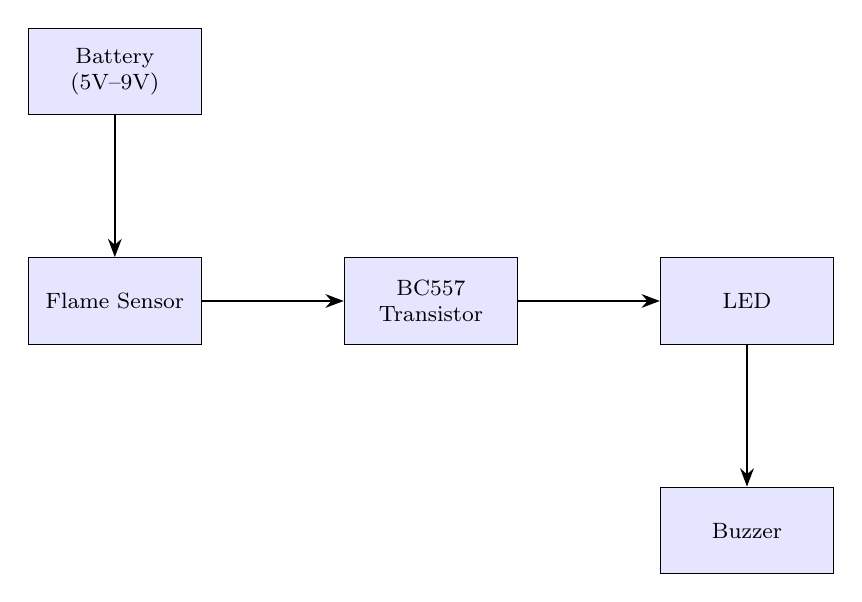
\begin{tikzpicture}[
			block/.style={rectangle, draw, fill=blue!10, minimum width=2.2cm, minimum height=1.1cm, text centered, align=center, font=\footnotesize},
			arrow/.style={-Stealth, thick},
			node distance=1.8cm
		]
		% Nodes
		\node[block] (sensor) {Flame Sensor};
		\node[block, right=of sensor] (transistor) {BC557\\Transistor};
		\node[block, right=of transistor] (led) {LED};
		\node[block, below=of led] (buzzer) {Buzzer};
		\node[block, above=of sensor] (battery) {Battery\\(5V--9V)};
		% Arrows
		\draw[arrow] (battery) -- (sensor.north);
		\draw[arrow] (sensor.east) -- (transistor.west);
		\draw[arrow] (transistor.east) -- (led.west);
		\draw[arrow] (led.south) -- (buzzer.north);
	\end{tikzpicture}
	\caption{Block diagram of the Fire Alarm using Flame Sensor and BC557 Transistor}
	\label{fig:block_diagram}
\end{figure}

\section{Circuit Diagram}
The circuit diagram of the fire alarm system is shown in Figure \ref{fig:circuit_diagram}. The flame sensor is connected to the base of the BC557 transistor, which acts as a switch. When the flame sensor detects fire, it sends a signal to the transistor, which then allows current to flow from the battery to the LED and the buzzer. The LED provides a visual indication of fire detection, while the buzzer emits an audible alert. The resistor is used to limit the current flowing through the LED and the transistor, ensuring that the components operate safely within their specified limits.

\subsection{Practical Circuit Diagram}
Figure \ref{fig:circuit_diagram} below shows the actual hardware connections for the fire alarm system. The flame sensor detects fire and sends a signal to the BC557 transistor, which activates the LED indicator and the buzzer. The buzzer provides an audible alert when fire is detected. The battery supplies power to the circuit. This practical setup allows us to test the functionality of the fire alarm system in real-world conditions and verify that it operates as intended when exposed to flames.

\subsection{Software Simulation Circuit Diagram}

Figure \ref{fig:software_circuit_diagram} below was created using TinkerCAD (or similar simulation software). It demonstrates the virtual setup and operation of the fire alarm system, allowing us to verify the design before practical implementation.

\begin{figure}[H]
	\centering
	\begin{subfigure}[t]{0.48\textwidth}
		\centering
		\includegraphics[width=\textwidth]{../Circuit Diagram.png}
		\caption{Practical circuit diagram}
		\label{fig:circuit_diagram}
	\end{subfigure}
	\hfill
	\begin{subfigure}[t]{0.48\textwidth}
		\centering
		\includegraphics[width=\textwidth]{../Software circuit diagram.png}
		\caption{Software simulation circuit diagram (TinkerCAD)}
		\label{fig:software_circuit_diagram}
	\end{subfigure}
	\caption{Circuit diagrams of the Fire Alarm using Flame Sensor and BC557 Transistor}
	\label{fig:circuit_diagrams}
\end{figure}

\section{Flow Chart}
The flowchart below illustrates the logical operation of the fire alarm system using a flame sensor, BC557 transistor, LED, and buzzer. It shows the sequence of steps from power-on to fire detection and alert.

\begin{figure}[H]
	\centering
	\includegraphics[width=0.8\textwidth]{../flowchart.png}
	\caption{Flowchart of the Fire Alarm System operation}
	\label{fig:flowchart}
\end{figure}

\section{Detailed Description}
The fire alarm system is a simple electronic circuit designed to detect the presence of fire and provide both visual and audible alerts. It uses a flame sensor to detect infrared radiation emitted by flames, a BC557 transistor as a switch, an LED for visual indication, and a buzzer for audible alert. When the flame sensor detects fire, it sends a signal to the BC557 transistor, which then activates the LED and buzzer.

The flowchart in Figure \ref{fig:flowchart} outlines the operation of the fire alarm system. The process begins with powering on the circuit. The flame sensor continuously monitors for the presence of fire. If no fire is detected, the system remains in a standby state. When the flame sensor detects fire, it sends a signal to the BC557 transistor, which then allows current to flow to the LED and buzzer. The LED turns on to provide a visual indication of fire detection, while the buzzer emits an audible alert to warn occupants of the potential danger. The system continues to operate until it is manually reset or powered off. This design ensures that the fire alarm system is responsive and effective in alerting individuals to fire hazards, enhancing safety in various settings.

The entire system is designed to be cost-effective and easy to maintain, making it accessible for use in homes, offices, and other buildings. The components used are readily available and the circuit can be easily assembled on a breadboard for testing and implementation.

\section{Results \& Analysis}
By implementing the fire alarm system in both software and hardware, the evaluation of performance is done. The results obtained from the testing phase are analyzed to assess the reliability and effectiveness of the fire alarm system. The key metrics evaluated include the Detection Reliability Index (DRI) and the average distance at which the system can reliably detect fire. The results obtained from the testing are as follows:

\subsection{DRI (Detection Reliability Index)}
The Detection Reliability Index (DRI) is calculated based on the number of successful detections of fire compared to the total number of tests conducted. In testing phase we conducted tests by changing and observed the response of the fire alarm system. The DRI is calculated and plotted in a graph as follows:

\begin{figure}[H]
	\centering
	\includegraphics[width=0.8\textwidth]{../DRI vs Distance-01.png}
	\caption{DRI vs Distance graph}
	\label{fig:dri_distance}
\end{figure}

\subsection{Average Distance Analysis}
The average distance at which the fire alarm system can reliably detect fire is calculated based on the results obtained from testing. The average distance is found to be approximately 15 cm, which indicates that the system is effective in detecting fire within a reasonable range. The results are plotted in the graph below:

\begin{figure}[H]
	\centering
	\includegraphics[width=0.8\textwidth]{{../Average Time vs Distance-01.png}}
	\caption{Average Time vs Distance graph}
	\label{fig:avg_distance}
\end{figure}

\subsection{Sensitivity Analysis}
The sensitivity of the fire alarm system is analyzed by adjusting the sensitivity of the flame sensor and observing the response of the system. The system is tested 5 times for $S_1$ = 0.0106 S/cm, $S_2$ = 0.018 S/cm, $S_3$ = 0.0206 S/cm, $S_4$ = 0.0054 S/cm and $S_5$ = 0.0126 S/cmsensitivity levels, \& the average sensitivity is calculated to be approximately 0.01344 S/cm.

\section{Conclusion}
In conclusion, the fire alarm system using a flame sensor and a BC557 transistor has been successfully designed, implemented, and tested. The system effectively detects the presence of fire and provides both visual and audible alerts. The results obtained from the testing phase indicate that the system is reliable and efficient in detecting fire hazards within a reasonable range. The average distance for reliable fire detection is approximately 15 cm, and the sensitivity analysis shows that the system can be adjusted to optimize performance. This project demonstrates the potential for creating cost-effective and accessible fire alarm systems that can enhance safety in various settings. Future work could involve further optimization of the circuit design, exploring additional sensors for improved accuracy, and integrating wireless communication for remote monitoring capabilities.

\section{Future Scope}
\begin{itemize}
  \item \textbf{Integration with Smart Home Systems:} The fire alarm system can be integrated with smart home systems to provide remote monitoring and control capabilities. This would allow users to receive alerts on their smartphones and take necessary actions even when they are not at home.

  \item \textbf{Use of Advanced Sensors:} Future iterations of the fire alarm system could incorporate advanced sensors such as smoke detectors, gas sensors, or temperature sensors to enhance the accuracy and reliability of fire detection.

  \item \textbf{Wireless Communication:} Implementing wireless communication technologies such as Wi-Fi or Bluetooth could enable the fire alarm system to communicate with other devices in the home, allowing for a more comprehensive safety network.

  \item \textbf{Energy Efficiency:} Future designs could focus on improving the energy efficiency of the fire alarm system, potentially by using low-power components or incorporating energy harvesting techniques.

  \item \textbf{Machine Learning for Fire Detection:} Incorporating machine learning algorithms could improve the system's ability to distinguish between actual fire hazards and false positives, such as steam or cooking smoke. This would enhance the reliability of the fire alarm system and reduce unnecessary alerts.
\end{itemize}

% References as numbered section at the end
\section{References}
\sloppy
\begin{enumerate}
	\item Z. Shafiq, R. Khan, M. Haseeb Zafar, G. Hafeez and R. A. Khalil, ``Optimal Placement of Fire Detection Sensors for Reduced Interference in Wireless Sensor Networks,'' \emph{IEEE Open J. Commun. Soc.}, vol. 6, pp. 9304--9321, 2025, doi: 10.1109/OJCOMS.2025.3626689.
	\item R. Elagib \emph{et al.}, ``Flame Detector Based on a Ge-on-Si Photodetector With a Voltage Tunable Spectral Response,'' \emph{IEEE Access}, vol. 13, pp. 174071--174077, 2025, doi: 10.1109/ACCESS.2025.3618306.
	\item M. M. E. H. Ali and M. Ghodrat, ``Toward Reliable Fire Detection in Indoor CCTV Footage: Reducing False Alarms From Benign Flames Using 3D Attention CNNs,'' \emph{IEEE Access}, vol. 13, pp. 144092--144103, 2025, doi: 10.1109/ACCESS.2025.3598919.
	\item M. Nakip, C. G{"u}zel{i}\c{s} and O. Yildiz, ``Recurrent Trend Predictive Neural Network for Multi-Sensor Fire Detection,'' \emph{IEEE Access}, vol. 9, pp. 84204--84216, 2021, doi: 10.1109/ACCESS.2021.3087736.
	\item A. H. Altowaijri, M. S. Alfaifi, T. A. Alshawi, A. B. Ibrahim and S. A. Alshebeili, ``A Privacy-Preserving IoT-Based Fire Detector,'' \emph{IEEE Access}, vol. 9, pp. 51393--51402, 2021, doi: 10.1109/ACCESS .2021 .3069588
\end{enumerate}
\end{document}
